%%%%%%%%%%%%%%%%%%%%%%%%%%%%%%%%%%%%%%%%%
% FRI Data Science_report LaTeX Template
% Version 1.0 (28/1/2020)
% 
% Jure Demšar (jure.demsar@fri.uni-lj.si)
%
% Based on MicromouseSymp article template by:
% Mathias Legrand (legrand.mathias@gmail.com) 
% With extensive modifications by:
% Antonio Valente (antonio.luis.valente@gmail.com)
%
% License:
% CC BY-NC-SA 3.0 (http://creativecommons.org/licenses/by-nc-sa/3.0/)
%
%%%%%%%%%%%%%%%%%%%%%%%%%%%%%%%%%%%%%%%%%


%----------------------------------------------------------------------------------------
%	PACKAGES AND OTHER DOCUMENT CONFIGURATIONS
%----------------------------------------------------------------------------------------
\documentclass[fleqn,moreauthors,10pt]{ds_report}
\usepackage[english]{babel}
\usepackage[T1]{fontenc}
\usepackage[utf8]{inputenc}
\usepackage{graphicx}

\graphicspath{{fig/}}




%----------------------------------------------------------------------------------------
%	ARTICLE INFORMATION
%----------------------------------------------------------------------------------------

% Header
\JournalInfo{Class: Natural Language Processing 2025}

% Interim or final report
\Archive{Project report} 
%\Archive{Final report} 

% Article title
\PaperTitle{Project 7: Analysis and comparison of translation errors and biases in LLMs} 

% Authors (student competitors) and their info
\Authors{Lea Vodopivec, Ines Kara\v{z}ija and Isabell Furkert}

% Advisors
\affiliation{\textit{Advisors: Ale\v{s} \v{Z}agar}}

% Keywords
\Keywords{Register-sensitive machine translation, Large language models (LLMs), Formality preservation, Prompt engineering, BLEU score}
\newcommand{\keywordname}{Keywords}


%----------------------------------------------------------------------------------------
%	ABSTRACT
%----------------------------------------------------------------------------------------

\Abstract{
	 This project investigates the ability of different large language models (LLMs) to preserve language register, especially when it comes to distinguishing formal and informal language. For this purpose, the FAME-MT corpus, a parallel English-German dataset that is already annotated for formality, was chosen and translated from English to Slovene as well. The evaluation focused on outputs from three LLMs (GPT-4o, DeepSeek and Gemma 3 27B) that were generated using various prompt strategies. The translations were then assessed using BLEU scores. Our findings show variation between LLMs and prompt types. However, GPT-4o consistently outperforms the other LLMs in translation and register sensitivity. Another finding is that explicit prompts lead to better results (although some models also handle implicit prompts well). While BLEU provides a good general insight into the translation accuracy, it fails to capture formality fidelity. 
}

%----------------------------------------------------------------------------------------

\begin{document}
	
	% Makes all text pages the same height
	\flushbottom 
	
	% Print the title and abstract box
	\maketitle 
	
	% Removes page numbering from the first page
	\thispagestyle{empty} 
	
	%----------------------------------------------------------------------------------------
	%	ARTICLE CONTENTS
	%----------------------------------------------------------------------------------------
	
	\section*{Introduction}
	The differentiation between formal and informal language registers play an important role in communication. However, machine translation systems still struggle to distinguish between them accurately [1]. This project examines how different Large Language Models (LLMs) handle register-sensitive translation, analysing their ability to adapt to formal and informal contexts, while identifying common errors and biases. Since control over formality is essential for producing natural and culturally appropriate translations, failures in this area can lead to awkward or even disrespectful output. Therefore, improving the ability of machine translation to manage formality remains a key challenge in natural language processing.
	European languages, such as English, Slovene and German, often express formality through complex syntax (e.g. subordinates clauses) or sophisticated vocabulary and phrasing.
	
	\section*{Related Work}
	A study conducted by Wang et al. [1] in 2023 explored the effectiveness of different prompting techniques to guide pre-trained LLMs such as GPT-3 and GPT by producing translations with controlled levels of formality. They introduce a robust Transformer-based classifier that outperforms previous evaluation metrics for formality-controlled translation. N\u{a}dejde et al. [2] also addressed the challenge of controlling formality in translations done by LLMs in their research. Their study highlights the issue of honorifics, using the example of translating \glqq{Are you sure?}\grqq into both formal and informal German. They introduce the CoCoA-MT dataset and an evaluation metric for training LLMs, demonstrating that fine-tuning on labeled contrastive data allows models to achieve high accuracy while maintaining translation quality. 
	In the work of Li \& Hu [3], the two researchers explore the “shining-through” effect in English translations from Chinese across four different registers, comparing human and machine translations. Their results show that the effect is present in both but more pronounced and persisted in machine-generated texts. The effect varies depending on the register, being most present in general and academic texts. 
	Mekki et. al [4] also contributed to the field of register-aware NLP by introducing the TREMoLo-Tweets corus, a large-scale French dataset of over 200 000 tweets annotated with labels based on their register. The project itself both demonstrates a way to automatically identify and analyze register in informal genres, such as social media, and provides a replicable framework for training register classifiers, which is relevant to evaluating register preservation in translated outputs as well. Moreover, the authors explore how linguistic descriptors (i.e. contractions, emoji use, verbal tense diversity) could be adapted to evaluate whether LLMs shift or preserve register when translating text between languages, and as such highlight the importance of capturing linguistic cues when evaluating whether an LLM translation maintains the tone, intention, and formality of the original.
	Similarly, Vela and Lapshinova-Koltunski [5] propose a register-based evaluation framework that incorporates lexico-grammatical features into the evaluation of machine translation output. By training classifiers on various linguistic characteristics, associated with different registers, they show that machine translations tend to share more register features with human translations than with original source text. This suggests that register awareness is often already implicitly handled during translation, but still not always consistently preserved across genres. Above all, their work emphasizes the need to evaluate machine-generated outputs in terms of how well they reflect the context and stylistic expectations of the source, not only based on content accuracy and similarity to the golden standard. Their findings also underscore the importance of assessing whether LLM-generated translations preserve or distort register, particularly when translating between formal and informal contexts.
	
	
	
	%------------------------------------------------
	
	\section*{Initial idea}
	The goal of our project is to analyse, assess and compare how large language models handle register variation when producing translations. We’re specifically interested into the distinction between formal and informal language and identifying whether and how these models preserve or shift the intended register of the source text across languages, genres and prompts. Through analysis, we would like to discover if certain models show a tendency toward a neutral, overly formal, or casual style.
	Our research will involve evaluating translation outputs from different LLMs across a range of text types, including both formal text (i.e. government proceedings) and informal (i.e. social media posts) language. We aim to assess the extent to which register is maintained or altered and under which circumstances, and to explore whether these shifts reveal any underlying biases or limitations in model behaviour. Ultimately, we seek to offer insight into strengths and weaknesses of current LLMs in handling stylistic variation in register.
	To evaluate the translation, register accuracy and variation, we will employ BLEU scores.
	% and human evaluations by native speakers who can assess the appropriateness and fluency of translated output in terms of register.
	
	
	\subsection*{Dataset \& Methods}
	
	\subsubsection*{Corpus Selection and Sampling}
	
For this project, we used the FAME-MT Corpus [5], a parallel dataset containing English and German sentence pairs annotated for formality level (formal vs. informal). This corpus was chosen for its diverse domains and explicit register labels, which allowed us to analyse the stylistic variation handled by LLMs during translation. 
To select a representative subset for analysis, we used the Orange Data mining toolkit, filtering the corpus to include only clearly labeled sentences, from which we randomly sampled 60 English sentences, ensuring a balanced distribution of 30 formal and 30 informal examples. In attempt to provide a rich testing ground, we sampled sentences that varied in tone, complexity and domain.

	\subsubsection*{Preprocessing and Reference Translation}
	
Before translation, we manually verified the German translations provided in the corpus to ensure they were appropriate and aligned with the intended register. Furthermore, we created human reference translations for the Slovene target language, as the FAME-MT Corpus does not provide Slovene translations. Each sentence was translated into Slovene by a native speaker, with a care to match the original sentence’s tone, vocabulary level, and syntactic structure, while still preserving fluency and meaning. These translations served as the gold standard for automatic BLEU evaluation later on.
All source sentences, human references and planned prompts were organized into a structured spreadsheet beforehand to facilitate systematic evaluation across multiple models and prompts. Alongside, we logged all translation outputs, prompt variants, source register, and evaluation metrics.

\subsubsection*{Translation Process and Prompts}

Later, each English sentence was translated into both German and Slovene using three different LLMs: ChatGPT (GPT-4o) [6], DeepSeek [7] and Gemma [8]. To evaluate how prompting influences register preservation as well, we developed four distinct prompt variants, categorized as Explicit A/B and Implicit A/B, each applied across both target languages. These prompt types were carefully designed to represent a range of prompt engineering techniques, from highly structured instructions to minimal guidance. 
		
\begin{itemize}
	\item Explicit A employed a few-shot instructional strategy, where the model was positioned as a certified translator and provided with three parallel examples. The prompt also clearly specified the model’s role and task constraints, instructing the model to be careful of register.
	\item Explicit B was designed as a chain-of-thought prompt, where the model was asked to identify the formality level, justify its judgement, and perform the translation, which encourages the model to reason about stylistic variation before generating output.
	\item Implicit A represents a few-shot prompt without any task instructions, rather relying solely on pattern induction by presenting example pairs of English sentences and their translations. While examples were given, no mention of the register was made.
	\item Implicit B follows a zero-shot approach with minimal instruction, forcing the model to infer both the task and its stylistic requirements from context.
\end{itemize}
	
\subsubsection*{Evaluation Methods}
To evaluate the performance of the translated outputs, we opted for a hybrid evaluation framework combining both automatic metrics and manual human evaluation. This approach allowed us to measure not only surface-level overlap, but also deeper aspects such as register preservation, fluency and semantic adequacy.
For quantitative evaluation, we used the BLEU score, a widely used metric for machine translation evaluation. At its core, BLEU computes the degree of overlap between the model-generated translation and a human reference by analyzing matching n-grams, and even though it is as such limited in its ability to capture stylistic variation, it remains useful for measuring general translation accuracy and consistency.
To compute sentence-level BLEU scores, we used the sacrebleu Python library. Each model output was evaluated against a gold-standard human reference translation, either from the FAME-MT corpus for German or our own manually created translations for Slovene. All BLEU scores were later stored in a structured evaluation spreadsheet for comparison across models, prompt types, registers and languages.
The criteria used for the human evaluation of the machine translated outputs in this project (i.e. formality, fluency, meaning preservation) were adapted from the methodology proposed by Rao and Tetrault in 2018 [6]. 



		\section*{Results}
		
	Our results highlight variations across models, prompt types and formality levels, revealing both the strengths and limitations of current LLMs in register-sensitive translation tasks. In the scope of analysis, the findings span the automatic BLEU scores, manual human evaluation and interpretation of both.
	
	\subsection*{BLEU Analysis}

		Overall, BLEU scores widely varied, with sentence-level scores ranging from as low as 3.6 to perfect scores of 100.
		
	\begin{figure}[h]
		\centering
		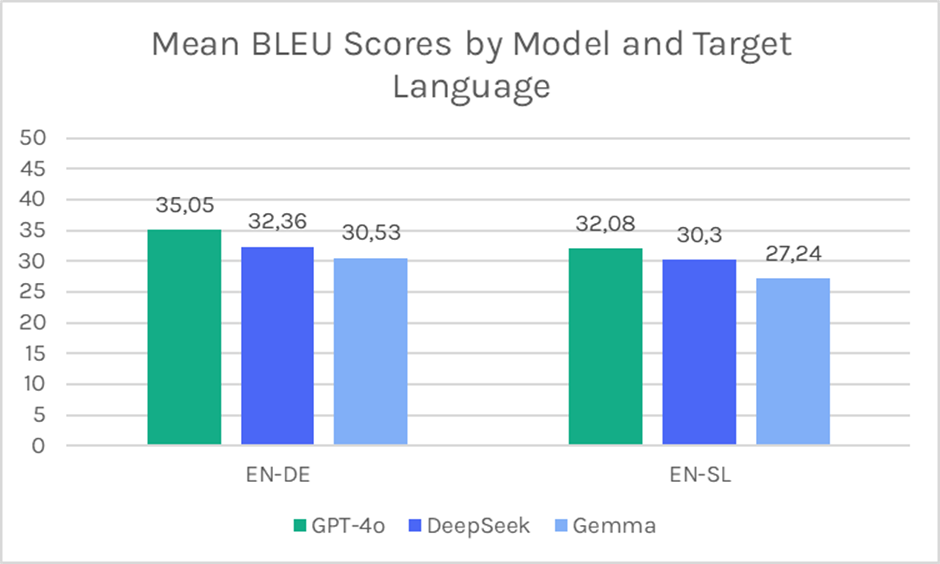
\includegraphics[width=0.5\textwidth]{image2.png}
		\caption{Mean BLEU scores for each model across German and Slovene translations}		
		\label{Figure 1}
	\end{figure}
		
	While the BLEU metric provides only a general indication of n-gram overlap with reference translations, we still managed to observe some patterns and key trends amongst the results.
	When analysing on language level, translations into German scored slightly higher on average than Slovene, which aligns with known limitations of BLEU in handling morphologically rich languages. Overall, the BLEU scores of the EN-SL sentence pairs showed more variability and a lower central tendency, which is likely due to word order flexibility and inflectional diversity in Slovene. The results may also reflect a broader trend in LLM training when referring to languages with enough digital coverage, like German, as opposed to those with less, like Slovene. Models are generally exposed to significantly more German data than Slovene, enabling more fluent and predictable output in EN-DE sentence pairs.
	Amongst the models, GPT-4o achieved the highest average and median BLEU scores, suggesting stronger lexical alignment with human references, again likely due to more advanced training and alignment techniques. On the other hand, DeepSeek, while occasionally performing well (especially in Slovene), showed wide variance, indicating unstable behaviour across sentence types and styles. Unfortunately, Gemma consistently underperformed in both language directions, with the lowest mean and median BLEU scores. Its outputs were often weaker or even grammatically incorrect, possibly due to limited stylistic data and domain-specific training.
	Although all models occasionally achieved perfect BLEU scores, only GPT-4o produced higher quality translations consistently. Nevertheless, all models demonstrated quite high variability, emphasizing their unreliability without fine-tuned control.
	
	\begin{figure}[h]
		\centering
		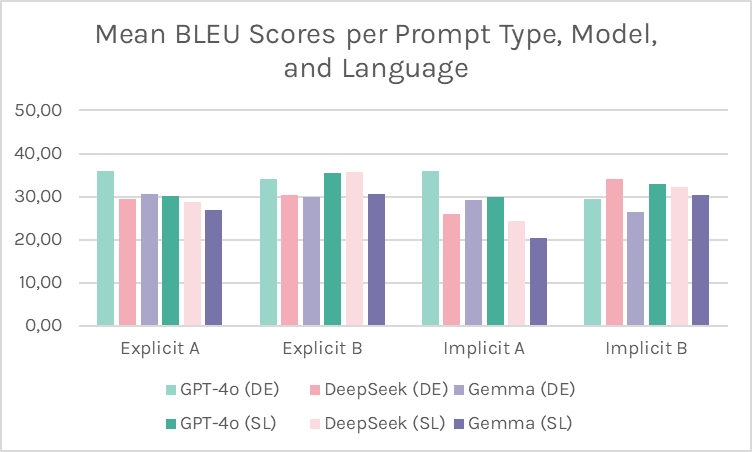
\includegraphics[width=0.5\textwidth]{image1.png}
		\caption{Mean BLEU scores by prompt type across three LLMs and two language pairs, where Explicit B results in the highest BLEU scores across nearly all systems, while Implicit A underperforms significantly}		
		\label{Figure 2}
	\end{figure}

Another factor that played quite a significant role in translation quality, the prompting strategy used. Prompt variants B consistently outperformed variant A, suggesting that improved prompt phrasing (e.g., step-by-step instructions, stronger contextual clues) aids model performance. In general, explicit prompts outperformed implicit ones as well, likely because they provided clearer guidance about stylistic and task goals. Notably, GPT-4o responded best to implicit prompts, particularly variant B, while DeepSeek and Gemma underperformed significantly on implicit prompts.


Register also interacted with prompt design: informal sentences were better translated using variant B, especially in implicit form, whereas explicit prompts, especially variant A, produced stronger results for formal inputs. Slovene translations generally performed worse under implicit prompting, reinforcing the importance of explicit guidance in languages as morphologically complex as Slovene.
Overall, we have discovered that GPT-4o appears to be the most register-sensitive model, benefiting from both implicit and explicit prompts depending on the context. This highlights the importance of prompt engineering as well: even small changes in wording can significantly influence output quality, especially with nuanced style when it comes to formal vs. informal input.
Despite these advances and insightful results, BLEU remains limited, as it does not account for register and punishes creative paraphrasing or stylistic shifts. For these reasons, we emphasize the continued importance of human evaluation in assessing register preservation as well.

		%------------------------------------------------
		
		\section*{Discussion}
		
Our study shows how LLMs handle register-sensitive translation but it also opens questions and ideas for future research. One of the main limitations in our research is the small dataset and language pairs that was chosen for our sample. Due to this relatively narrow scope, this study is too limited to generalize conclusions about each model's performance. Furthermore, our analysis is restricted to only a handful of prompt variations. Future studies could investigate more prompting methods that guide the LLMs so that it's more sensitive to the specific inputs. This could lead to a better preservation of the register-style and improve the general quality of the translation. Another potential improvement would be to integrate more register-sensitive evaluation metrics since our findings showed that BLEU scores alone cannot fully capture the stylistic nuances. Tools like automatic classifiers or human evaluation methods could help providing a more accurate assessment of register preservation. 
Finally, our research focused on general-purpose LLMs while there is also a lot of potential in exploring how domain-specific or fine-tuned models translate register-sensitive context and whether they could outperform the other LLMs. Nevertheless, analysing and improving register preservation is essential in machine translation systems since they are deployed in increasingly contextually sensitive settings.
		
		
		%------------------------------------------------

		
		
		
		
		%----------------------------------------------------------------------------------------
		%	REFERENCE LIST
		%----------------------------------------------------------------------------------------
		\bibliographystyle{unsrt}
		\bibliography{report}
		\renewcommand{\labelenumi}{[\theenumi]}
		\begin{enumerate}
			\item  P. C. Wang, E. Marrese-Taylor, Y. Matsuo, “Prompting pre-trained Large Language Models for formality-controlled En-Ja Translation”, in 人工知能学会全国大会論文集, vol. JSAI2023, pp. 2E5GS602-2E5GS602, 2023.
			\item M. N\u{a}dejde, A. Currey, B. Hsu, X. Niu, M. Federico and G. Dinu, "Cocoa-mt: A dataset and benchmark for contrastive controlled mt with application to formality," 2022.
			\item Y. Li, “A better or worse communicator? Comparing human and machine translation in source language shining through across registers”, in Lingua, vol. 312, p. 103834, 2024.
			\item J. Mekki, G. Lecorvé, D. Battistelli, N. Béchet, “TREMoLo-tweets: A multi-label corpus of French tweets for language register characterization”, in RANLP 2021-Recent Advances in Natural Language Processing, Sept. 2021.
			\item D. Wisniewski, Z. Rostek, and A. Nowakowski, "FAME-MT Dataset: Formality Awareness Made Easy for Machine Translation Purposes," in Proceedings of the 25th Annual Conference of the European Association for Machine Translation (EAMT), Sheffield, UK, pp. 164–180, 2024.
			\item OpenAI, ChatGPT (Version 14. März) [Large language model (bzw. Großes Sprachmodell, Anm.)]. https://chat.openai.com/chat, 2023.
			\item DeepSeek, DeepSeek LLM: An open-source language model, https://deepseek.com, 2024.
			\item Google, Gemma: Open models from Google DeepMind, https://ai.google.dev/gemma, 2024.
			\item S. Rao and J. Tetreault, "Dear sir or madam, may I introduce the GYAFC dataset: Corpus, benchmarks and metrics for formality style transfer," arXiv preprint, arXiv:1803.06535,2018.
		\end{enumerate}
		
		
	\end{document}